%!TEX TS-program = xelatex
%!TEX encoding = UTF-8 Unicode
\documentclass[11pt, a4paper]{article}

\usepackage{fontspec, xunicode, xltxtra}
\defaultfontfeatures{Mapping=tex-text}
\setmainfont{Adobe Caslon Pro}
\setmonofont[Scale=MatchLowercase]{Monaco}
\setmathrm{Cambria Math}

\usepackage{paralist} % for better itemize and enumerate
% asparaenum, inparaenum, \begin{compactenum}[{Example} a)] etc.
% Also, items can be referenced via \label{} and \ref{}
%
\frenchspacing
\usepackage{natbib}
\bibpunct{(}{)}{;}{a}{,}{,}
\usepackage{gb4e}
\usepackage{wrapfig}

\title{Thesis Notes}
\author{\textsc{Pavel Straňák}}

\begin{document}
\maketitle

%%%%%%%%%%
\subsection*{Idioms}
Even ``non-compositional'' idioms are actually (originaly) metaphorical or methonymical.  Even though sometimes it is hard to see that. At other times a speaker may forget that rather straightforward metaphoric aspect:

\begin{quote}
Barack Obama accused his Republican rivals of stirring a controversy over a comment he made about putting “lipstick on a pig.” \emph{(NY~Times, 11.~September 2008)}
\end{quote}


%%%%%%%%%%%%%%%%%%%%%%%%%%%%%%%%%%%%%%%
\section{PDT 2.0}\label{PDT}
In PDT there are several functors that refer to multiword expressions (MWEs) in one way or another. There are also some technical lemmas (??? nebo jen 1?) like {\tt \#Forn} that identify roots of subtrees representing MWE's.

There are currently two graphical search engines for PDT: Netgraph \cite{netgraph} and TrEd \cite{tred}. Both have their respective benefits, but since TrEd is considerably faster due to its use of an SQL database backend \cite{pmltq}, we have used TrEd for all the examples in this work. We also give the search queries using the PML Tree Query language \cite{pmltq} where appropriate.

%%%%%%%%%%
\subsection{Foreign Phrase: \tt{t-node [t\_lemma = \#Forn]}}\label{PDT:Forn}
Foreign Phrase seems to be overused and its overuse seems a bit arbitrary. \\
- jmena firem jsou nekdy forn, nekdy ne. (dohledat)\\

%%
\subsubsection{Foreign phrases with just one t-node}
There are 34 occurrences of this construction in the PDT~2.0. Counting them is as easy as writing a query in Figure~\ref{fig:tq-forn1} and extending it with this filter: \texttt{>>count(\$n)}.

\begin{wrapfigure}{r}{0.32 \textwidth}
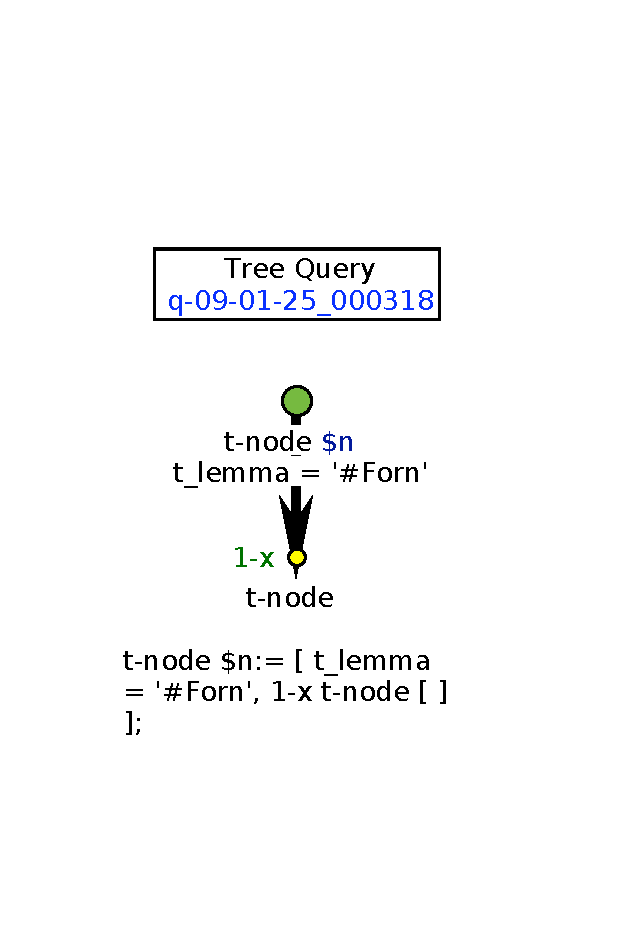
\includegraphics[width=0.3 \textwidth]{vyhledavky/query-forn-1-x.pdf}
\caption{PML-TQ search query for single-node foreing phrases}
\label{fig:tq-forn1}
\end{wrapfigure}

In case of the bibliographic reference in Figure~\ref{fig:forn-biblio} there is coordination of three foreign phrases corresponding to the parts of a bibliographic reference annotated, but the reason for this is not very clear. After all, the point of annotating foreign phrases as simple lists with a {\tt \#Forn} node as a head was to make no assumptions about these pieces of a text \pageref{pdt-t-man:300}.  \\
- je to kvuli te interpunkci???

\begin{figure}[h]
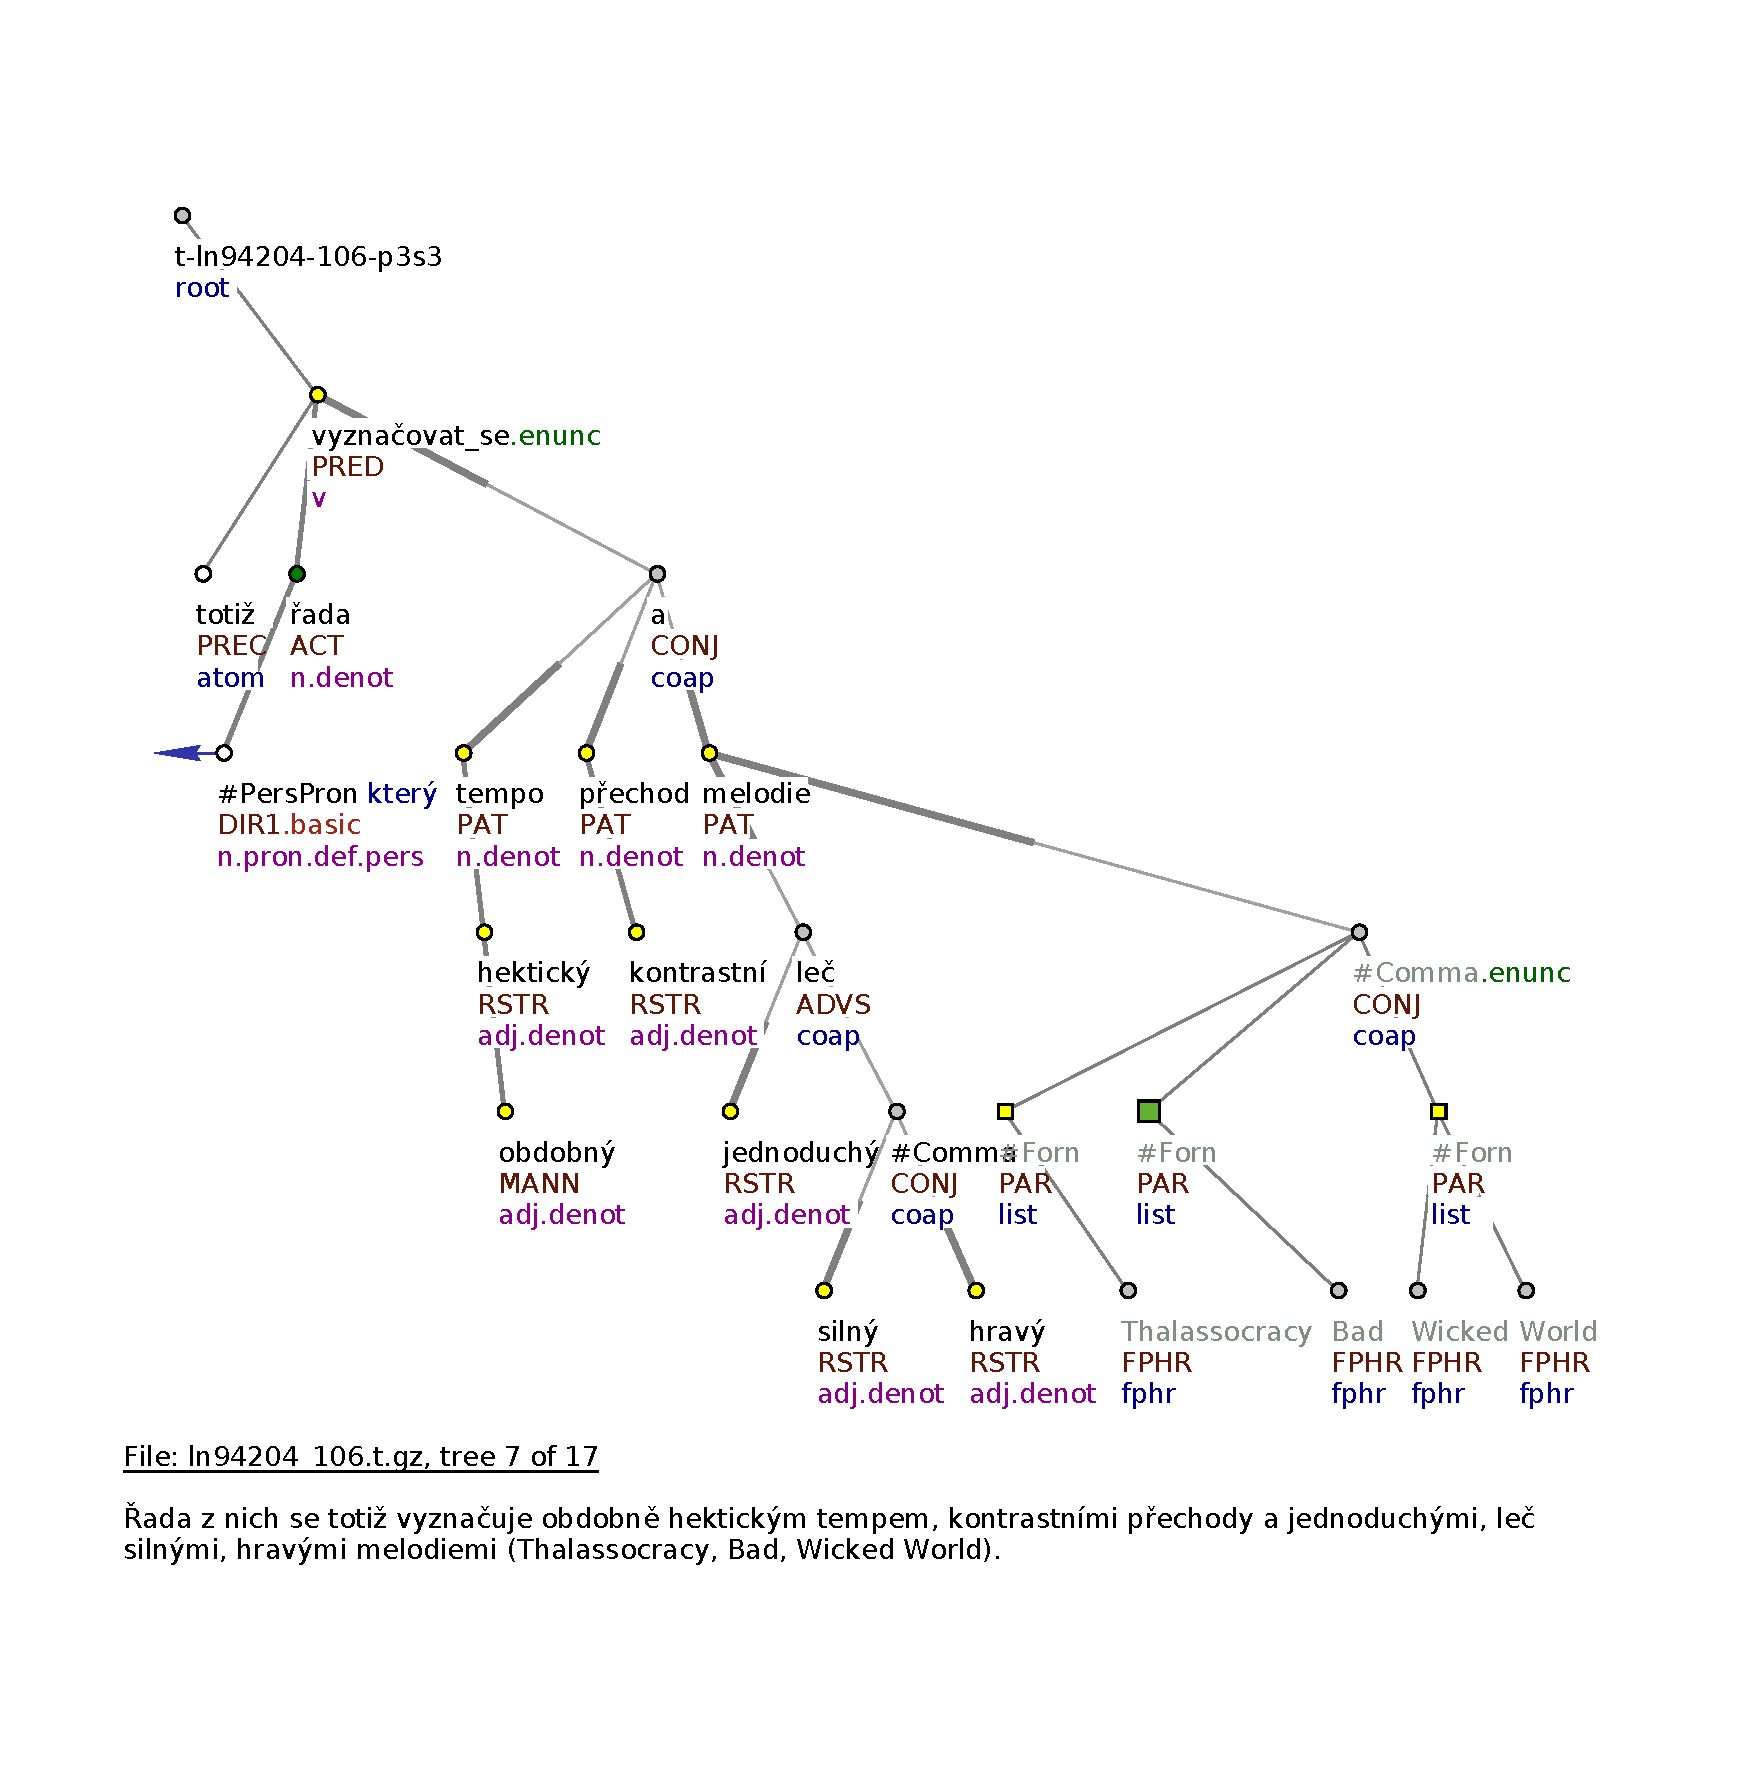
\includegraphics[width=\textwidth]{vyhledavky/forn-coord1x-biblio.pdf}
\caption{A bibliographic reference analysed as a coordination of three foreign phrases}
\label{fig:forn-biblio}
\end{figure}

Names of companies seem to be distinguished more by the country of origin then by any linguistic reasons, as demonstrated in Figure~\ref{fig:forn-firmy}. As far as linguistic criteria are concerned, Chemapol and Inekon are as foreign as Agip or Total. However the first two are, or at least were%
\footnote{At the time of writing this thesis Chemapol is owned by another international company, which only emphasises vagueness of this distinction} %
%
, Czech companies, while those in the latter group have a foreign origin.

\begin{figure}
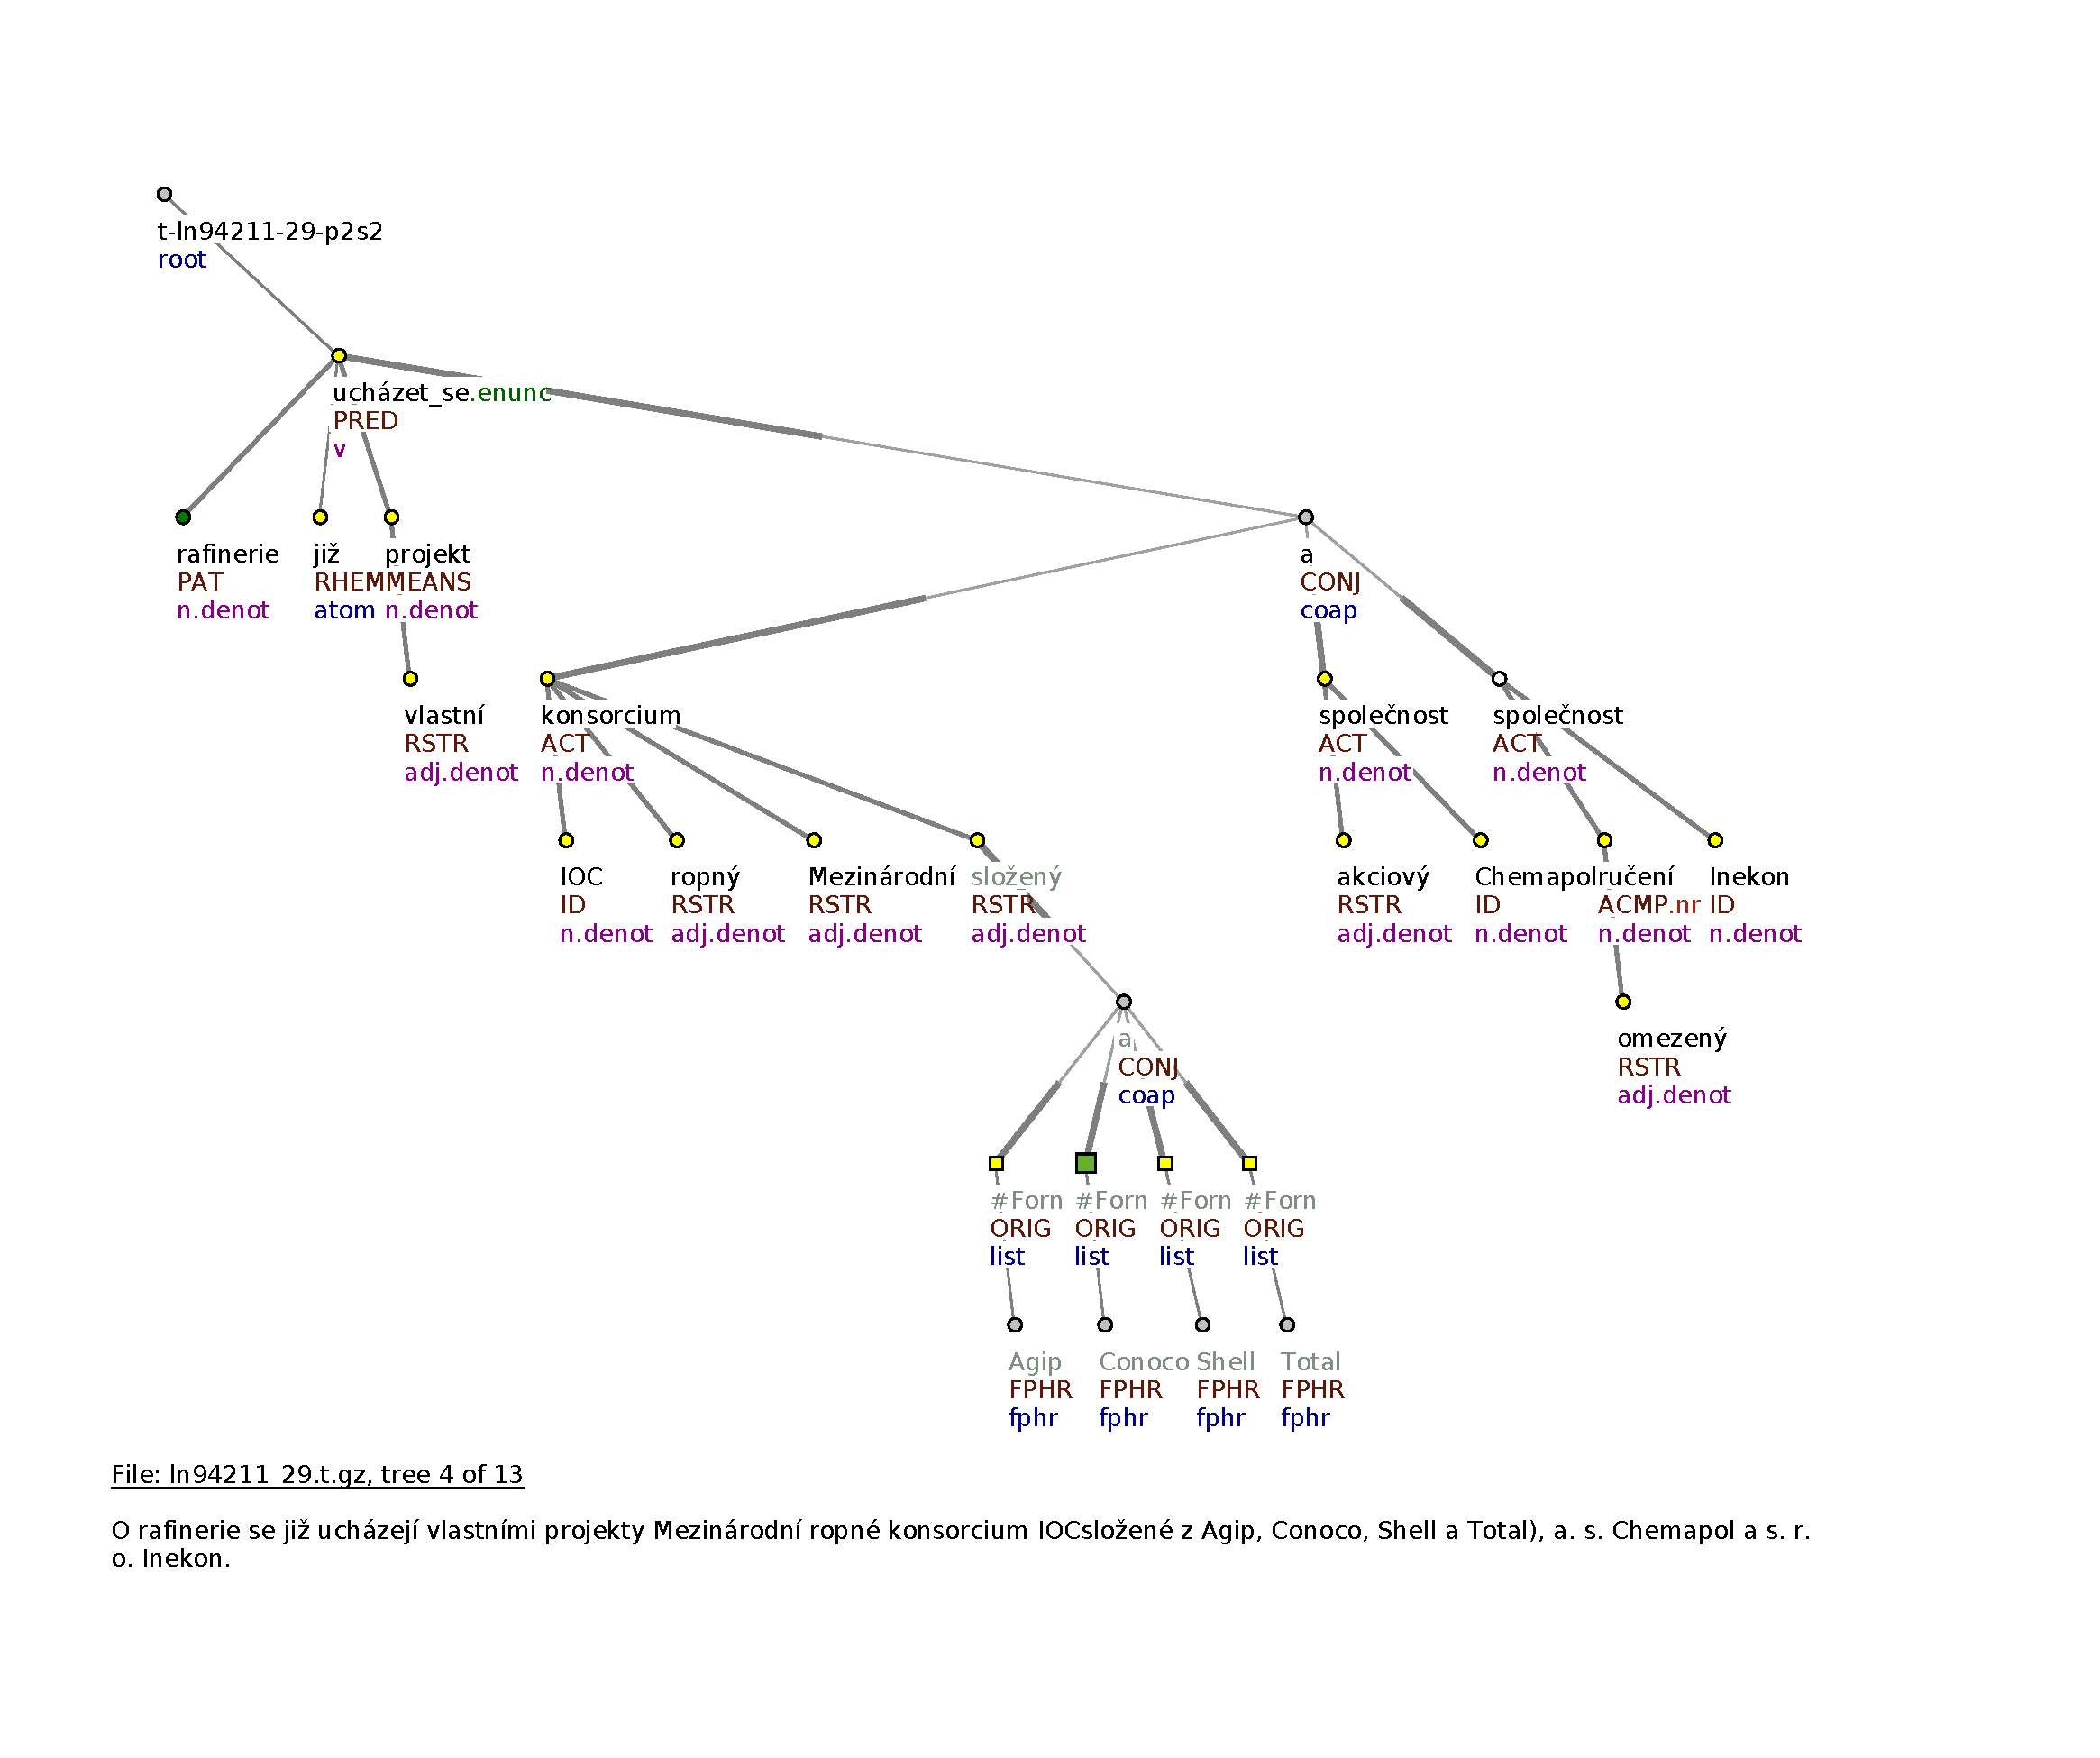
\includegraphics[width=\textwidth]{vyhledavky/nazvy-firem.pdf}
\caption{Annotation of Czech and foreign company names}
\label{fig:forn-firmy}
\end{figure}

%%%%%%%%%%
\subsection{CPHR}
There are 76 occurrences of {\tt CPHR} nodes, whose head verb is not its parent, but only effective parent, in 40 sentences. See Figure~\ref{fig:tq-echild} for the query and Figures~\ref{fig:cphr-echild} and~\ref{fig:cphr-echild2} for examples.
\begin{wrapfigure}{r}{0.32 \textwidth}
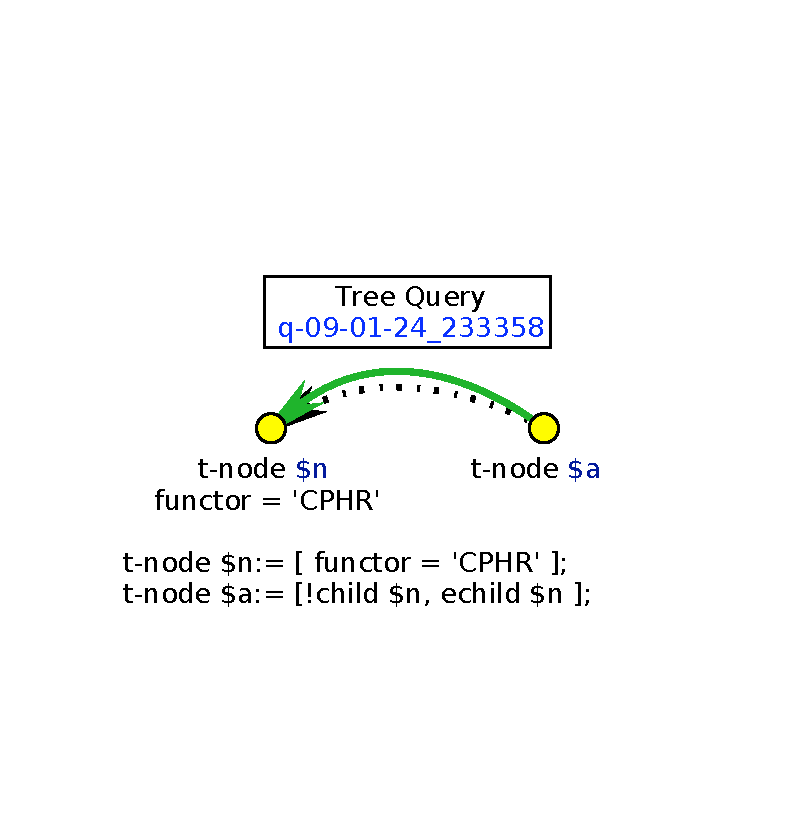
\includegraphics[width=0.3 \textwidth]{vyhledavky/query-echild.pdf}
\caption{PML-TQ search query for CPHR nodes, whose effective parrent is not its parent}
\label{fig:tq-echild}
\end{wrapfigure}

\begin{figure}[h]
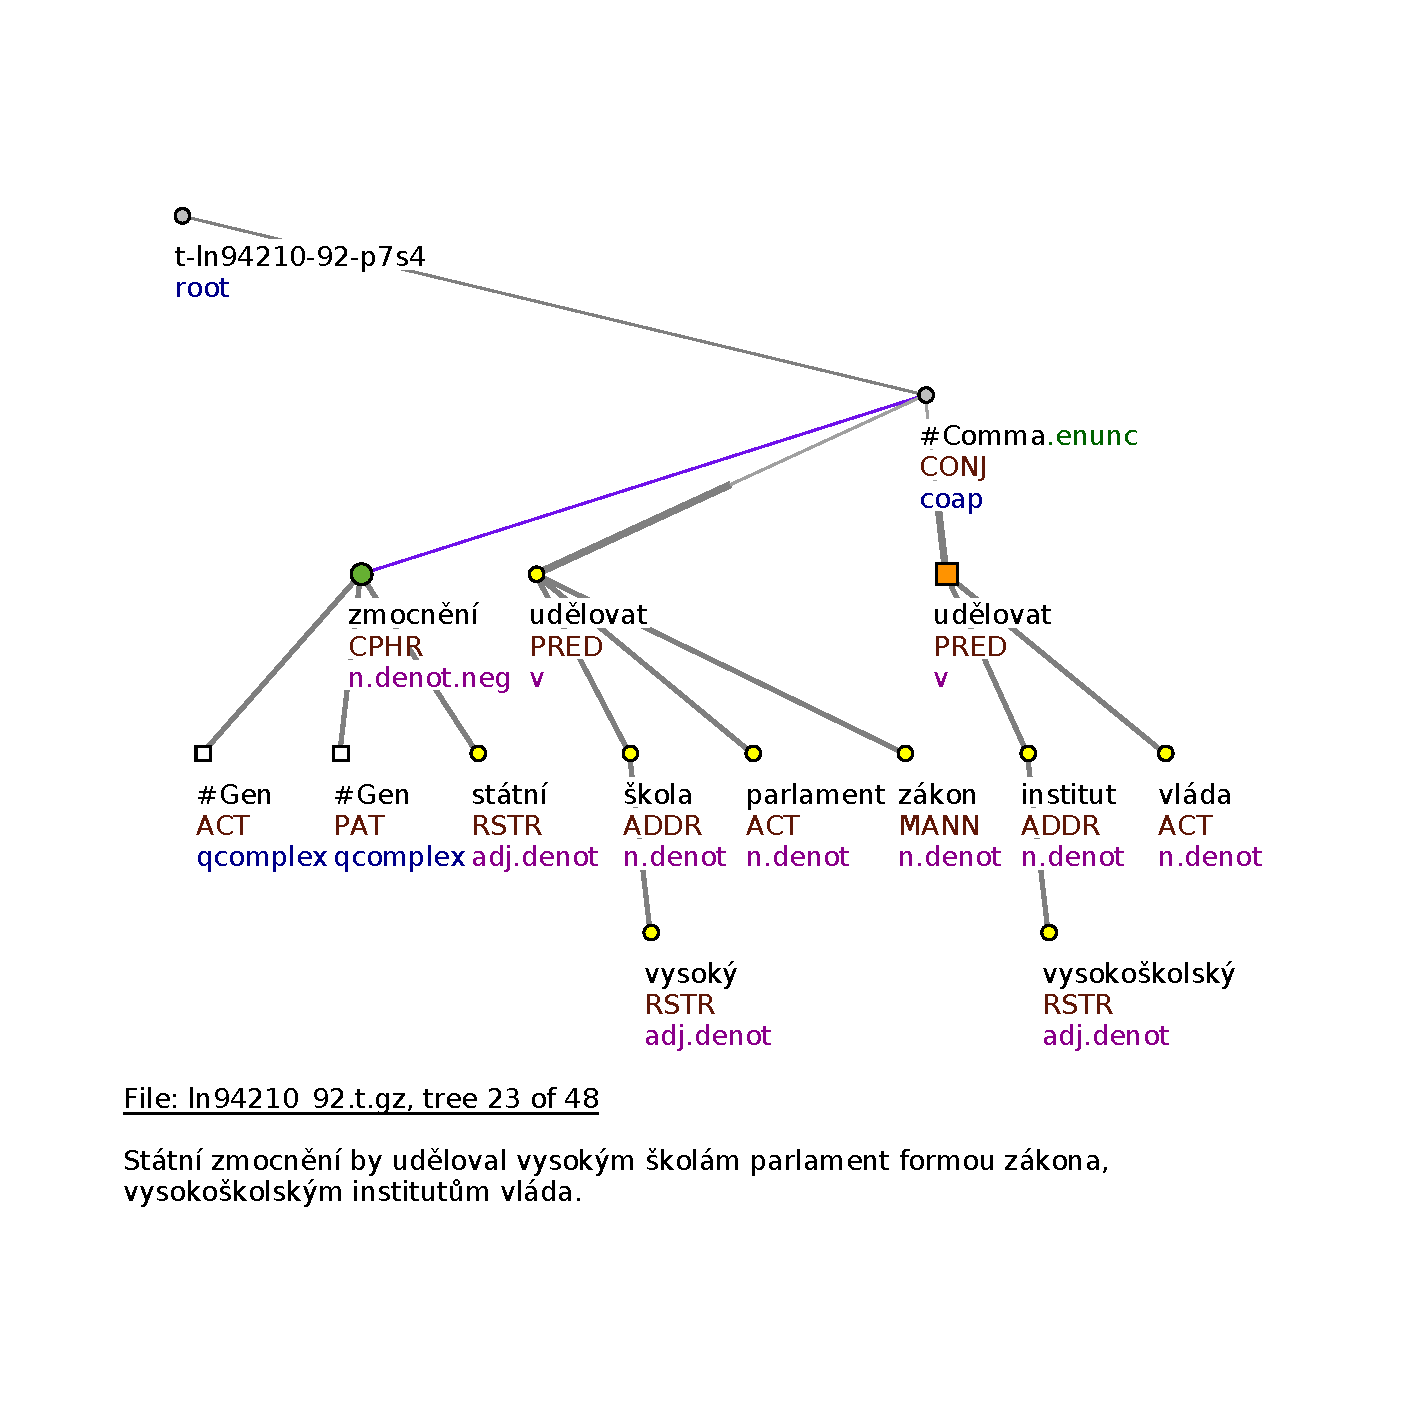
\includegraphics[width=0.8\textwidth]{vyhledavky/cphr-echild.pdf}
\caption{Coordination of verbonominal idioms, where the verbal parts are further ???rozvite }
\label{fig:cphr-echild}
\end{figure}

Figure~\ref{fig:cphr-echild2} shows on the other hand a coordination of two V-N idioms with the same verbal part.
\begin{figure}[h]
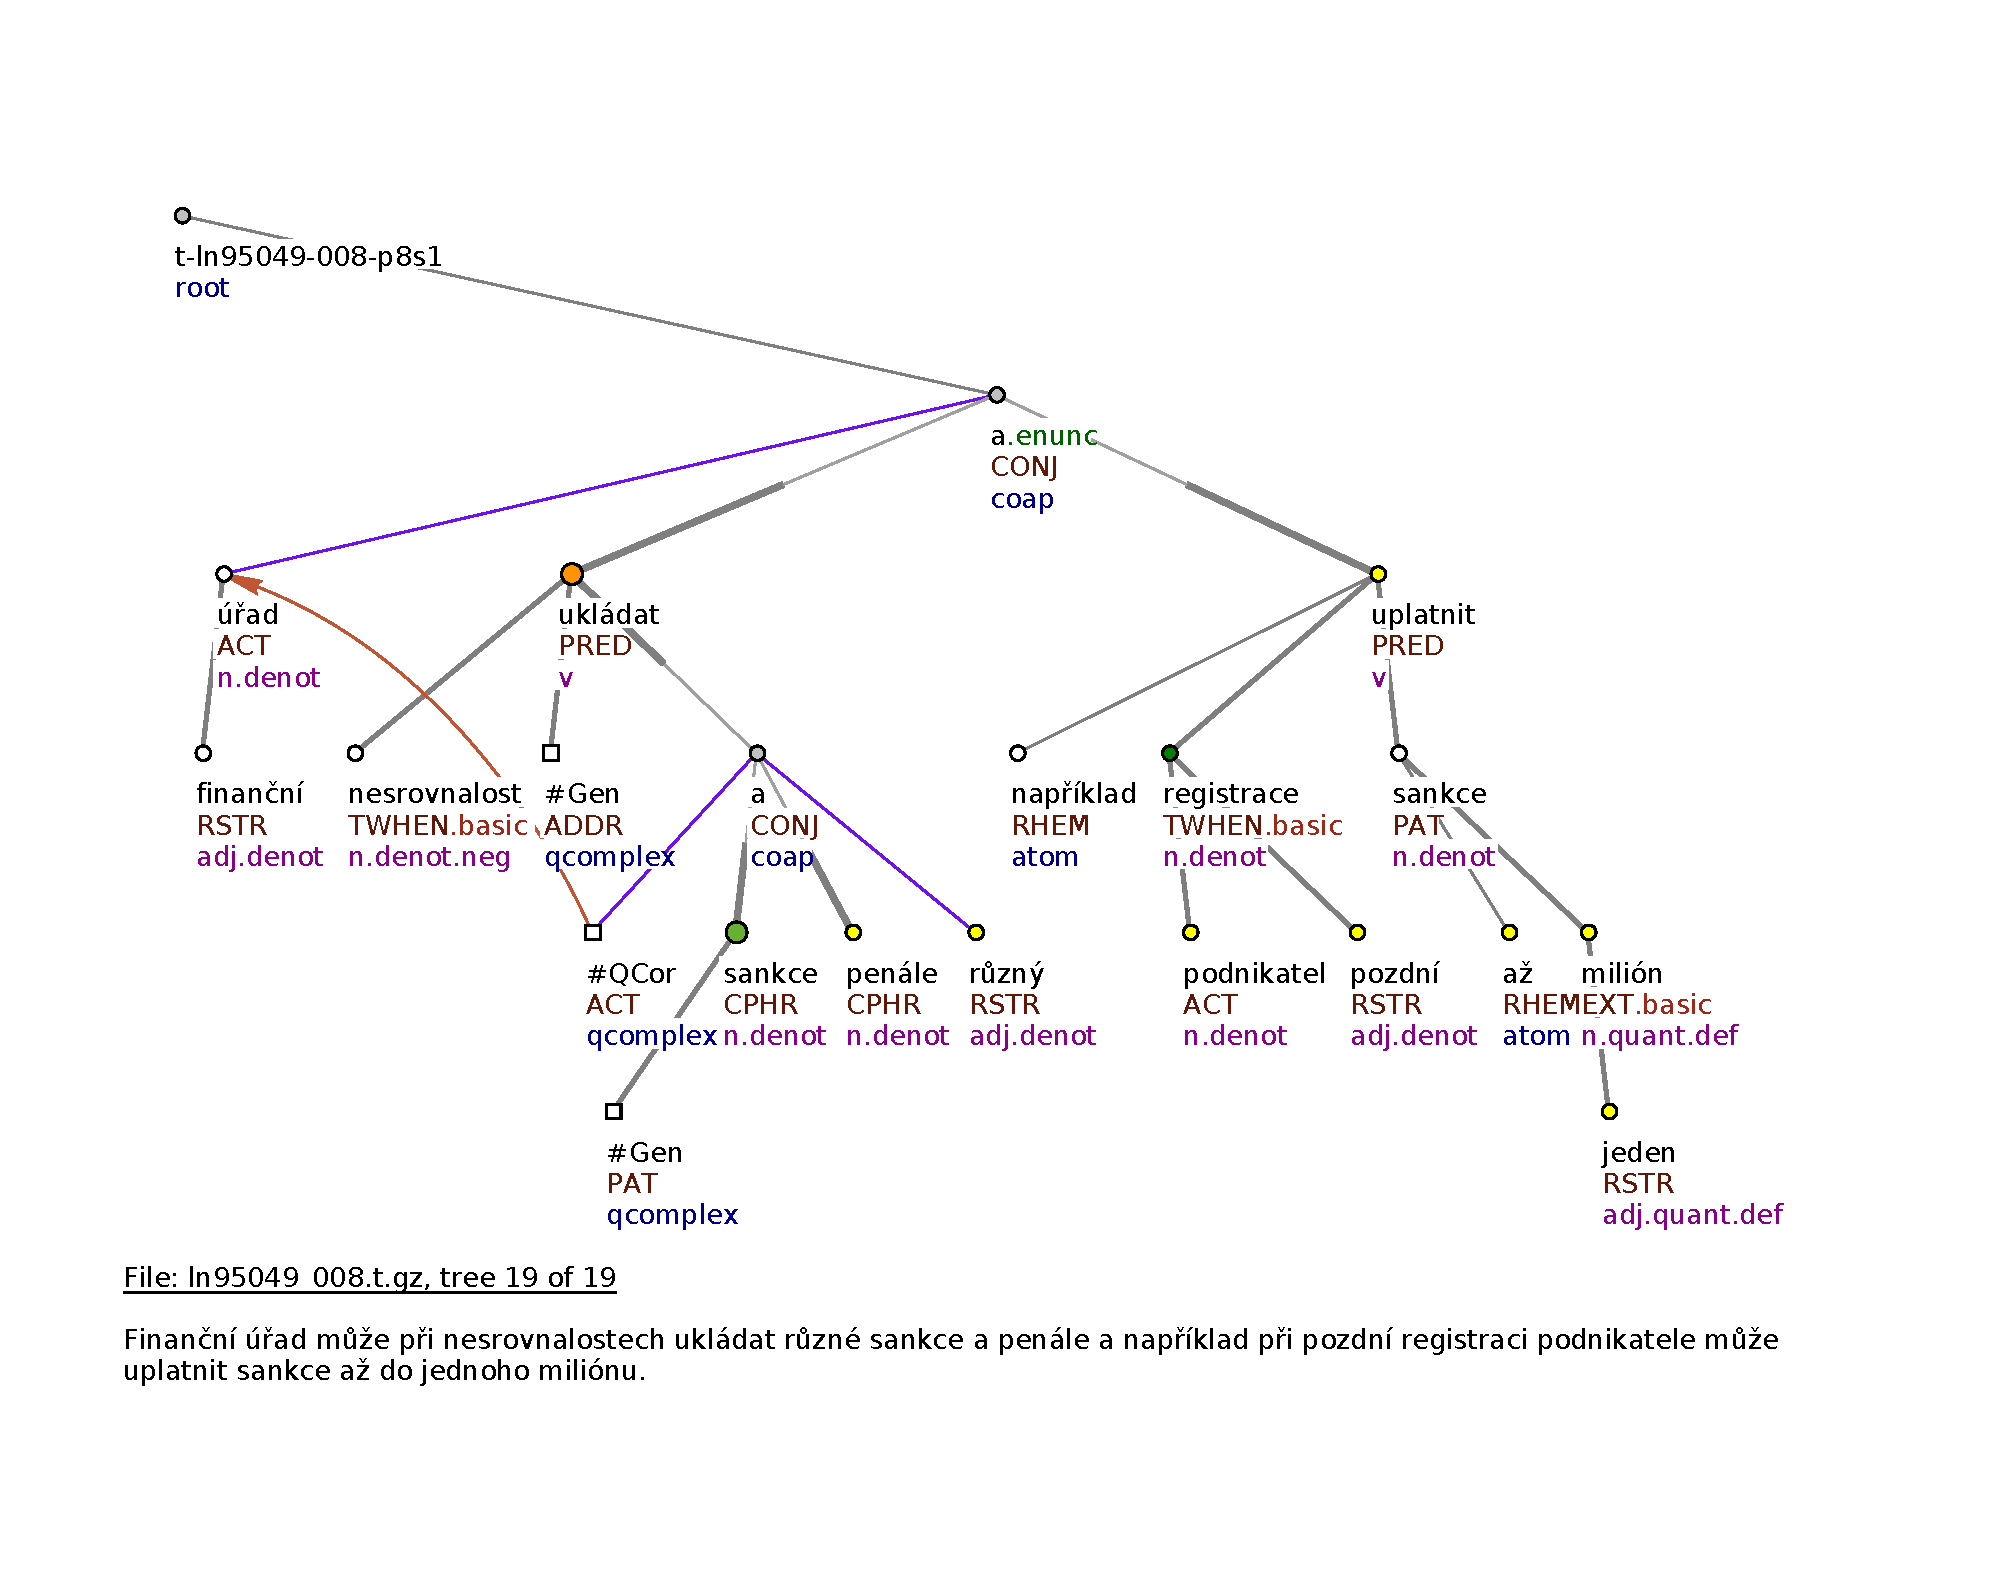
\includegraphics[width=\textwidth]{vyhledavky/cphr-ukladat-sankce-a-penale.pdf}
\caption{Coordination of two idioms starting with the same verb}
\label{fig:cphr-echild2}
\end{figure}


\bibliographystyle{plainnat}
\end{document}